We used a number of tests to validate the code. There are a number of unit tests designed to test individual functions in the code. For integration testing we selected a suite of simple problems all using a single material on a square domain for which we could derive or approximate analytic solutions. We varied the material properties to trigger use of the various solvers. These problems were a single energy group with no scattering, a single energy group with scattering, and two energy groups with scattering. 

\section{NDA/SAAF Agreement}
We also tested the agreement between the NDA+SAAF and SAAF alone to ensure we were replicating expected behavior. Based on previous studies we do not expect the two methods to perfectly agree with each other \cite{morel-holo}. However, the two solutions should approach each other as the number of mesh cells increases \cite{Wang2013}. We simply compare the mean difference in the SAAF and NDA solutions for scalar flux as number of mesh cells increases. We notice the two solutions approaching each other as the number of mesh cells increases. 
\begin{figure}[H]
    \centering
    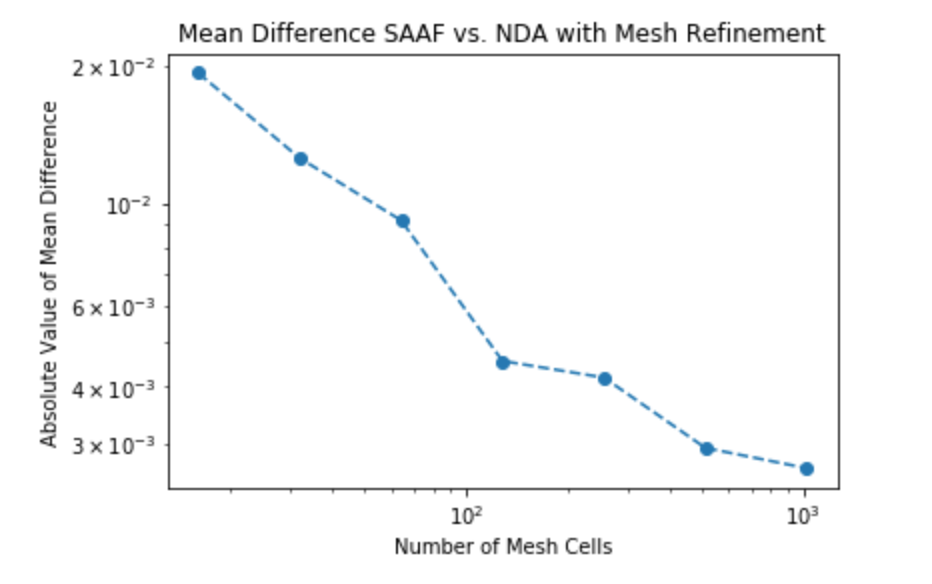
\includegraphics[width=.75\textwidth]{fig/NDAvsSAAF.png}
    \caption{SAAF/NDA Agreement with Mesh Refinement}
    \label{fig:SAAFvsNDA}
\end{figure}



Finally, we plot a 1-D line out of all three methods. For this problem we chose one test material with one group and some scattering. This is more of a gut check than a formal check of convergence. From this plot we can clearly see that NDA has provided a correction to diffusion, producing a solution that is much closer to the higher order equation than diffusion by itself. 

\begin{figure}[H]
    \centering
    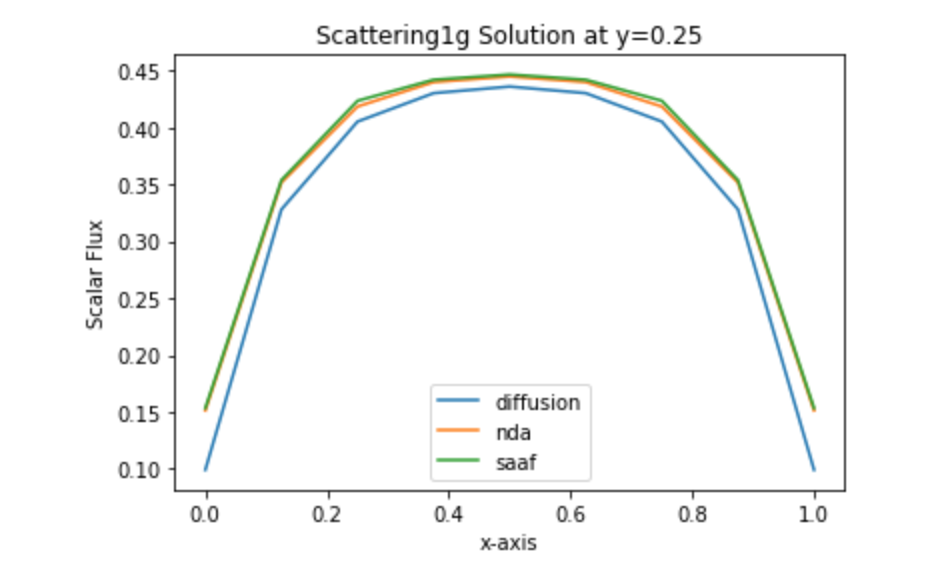
\includegraphics[width=.75\textwidth]{fig/LineOut25.png}
    \caption{Comparison of Diffusion, SAAF, and NDA}
    \label{fig:comparison}
\end{figure}

From the results of these three checks, we determine that we are in agreement with previously published work on SAAF+NDA and have implemented a working version. 